\section{Introdução}

Este documento é um guia com orientações para o uso de slides em apresentações a serem feitas pelos laboratórios LUDES e LINE, no Programa de Engenharia de Sistemas e Computação da COPPE/UFRJ. Devem ser úteis a outros grupos.

Ele é construído como um guia básico, e razoavelmente conservador.

Este material está disponível no GitHub, junto com material de apoio, como slides Power Point que eu uso e distribuo: \url{https://github.com/xexeo/DicasSlidesAcademicos}.

Outra questão importante neste documento: ele é criado por um usuário do \textit{Power Point} que tem pouca experiência com o \texttt{beamer}, o estilo de apresentações do \LaTeX. Muitos softwares de apresentação são altamente compatíveis com o \textit{Power Point}, seguindo a mesma filosofia de trabalho, baseado no WYSIWYG. Outros softwares, como o Prezi\footnote{\url{https://prezi.com/}} podem exigir outra forma de pensar, porém muitas dicas dadas aqui continuam válidas. A Seção \ref{sec:ferramentas} discute um pouco os principais softwares e características importantes do seu uso.

Usarei o termo geral \textit{apresentação} para uma aula, defesa de tese ou apresentação de artigo em congresso.

Os slides são impressos com frames gerados no \LaTeX\ para delimitar o seu tamanho, os frames não fazem parte dos mesmos, podendo ser gerados de outra forma por outros aplicativos.

Outra questão: todos os slides apresentados são reais, e quebram algumas vezes minhas sugestões. Por exemplo, os slides feitos com \texttt{beamer} usam números pequenos, o que é uma característica do tema Lubeck. Já os slides de \textit{Power Point} muitas vezes não possuem o número total de slides, porque isso dá mais trabalho do que deveria nesse software.

\subsection{Filosofia dos Slides}

Os ``slides'' são uma ferramenta usada em apresentações há muitos anos, sendo substitutos digitais de outras formas de apresentação, como quadro negro, posters, fotografias, projeções com slides (do tipo filme), transparências, etc. Muitos autores famosos questionam o uso de softwares como o PowerPoint para a criação de slides, ou mesmo para a apresentação de projeto e aulas, porém não há como negar que eles são práticos, facilmente criados e usados universalmente.

Este guia segue uma filosofia: o trabalho de criar os slides não pode ser grande. Além disso, eles devem ajudar tanto o professor a passar sua mensagem, mas também ao aluno a acompanhar a aula, entender o material, e poder usá-lo mais tarde.

Para isso, os slides não podem ser nem entendiante, nem levar o aluno a se dispersar, ou se perder tamanha a quantidade de informações. Isso se aplica tanto a um slide isolado, quanto a uma sequência de slides.

Além disso, devem ser criados para atender não só um assistência normal, mas também os que tem alguma dificuldade, como visualização de cores, dificuldade de leitura a distância e mesmo dificuldades auditivas (nesse caso, o slide deverá conter informação suficientes para ajudar que assiste a entender o assunto).

Nossa filosofia parte da ideia de 4 tipos de slides padrão: o de título, o slide de texto, o slide de imagem e o slide de texto e imagem. A partir desses tipos, várias variações podem ser criadas.

\begin{figure}[hbt]
    \centering
    \subfloat{
        
\includegraphics[width=0.4\linewidth,frame]{Slides/tiposbasicos/Slide1}}
    \subfloat{
        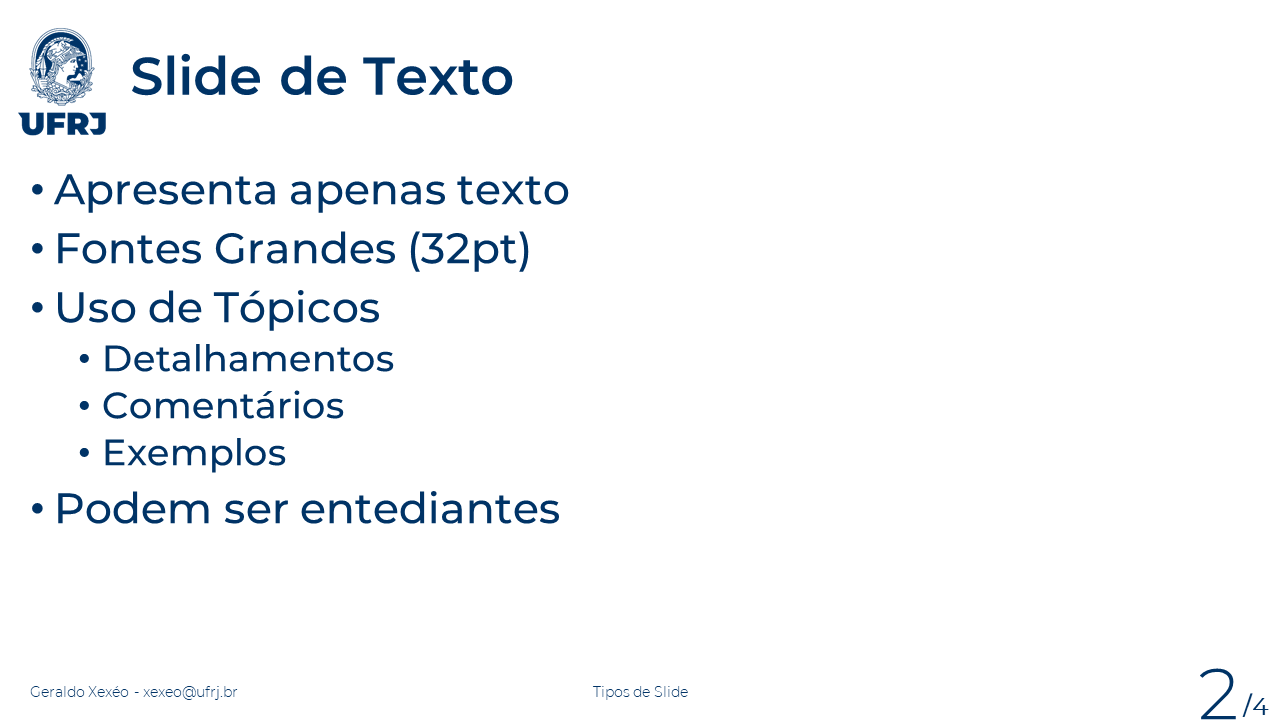
\includegraphics[width=0.4\linewidth,frame]{Slides/tiposbasicos/Slide2}}\\
    \subfloat{
    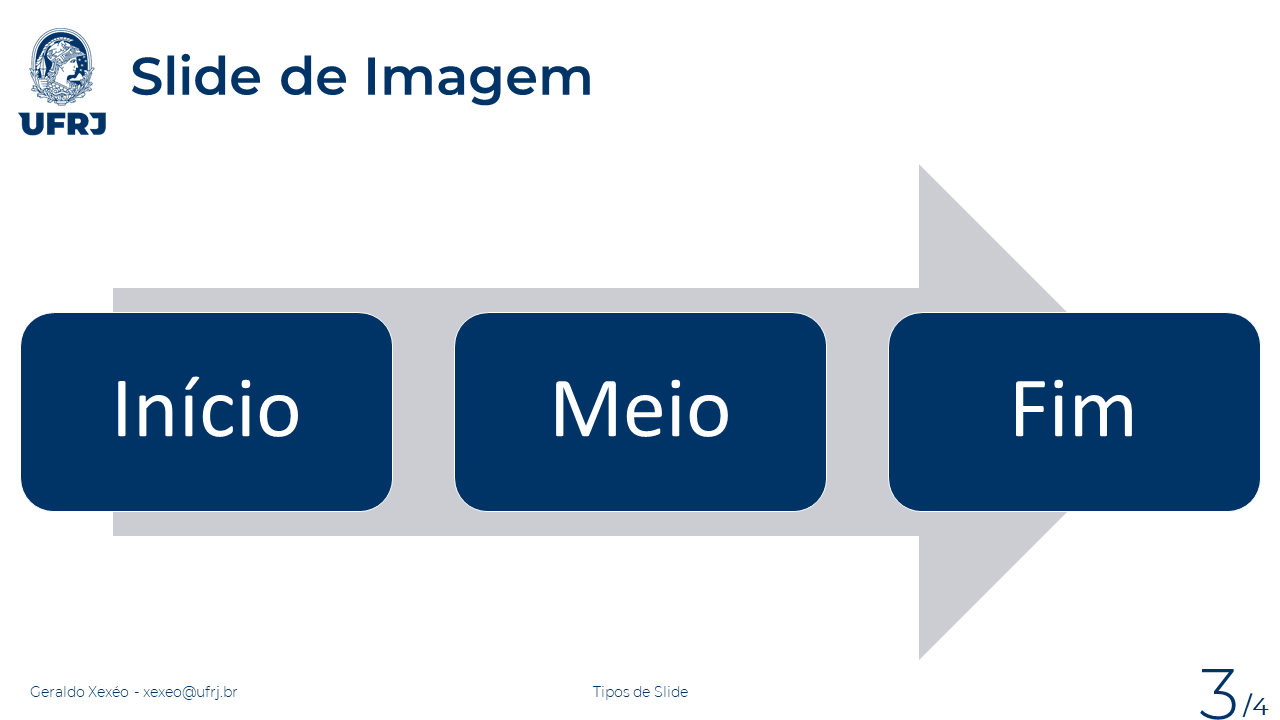
\includegraphics[width=0.4\linewidth,frame]{Slides/tiposbasicos/Slide3}}
    \subfloat{
    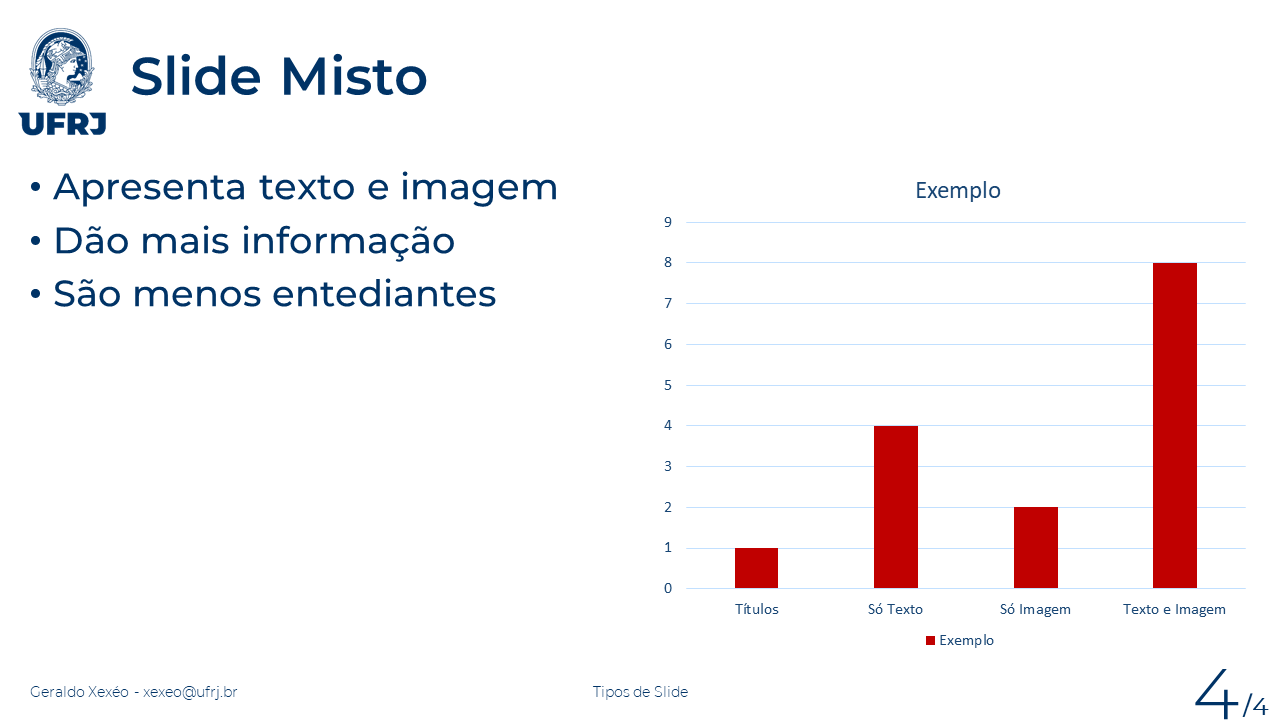
\includegraphics[width=0.4\linewidth,frame]{Slides/tiposbasicos/Slide4}}
    \caption{Tipos básicos de slides.}
    \label{fig:tiposbasicos}
\end{figure}

Outra premissa desse texto, que dificilmente pode ser discutida, é que a apresentação é feita, pelo professor ou apresentador, na forma de uma narrativa linear. Mesmo que use truques de apresentar algo antes, ou deixar algo para mais tarde, de qualquer forma, a narrativa será feita, durante a apresentação, passo a passo. Voltar a trás, dar ``hiperpulos'' com o texto só causa confusão a plateia.

\subsection{Outras ferramentas}

Existem outras ferramentas que propõe o que seriam novas formas de fazer apresentações, organizando a apresentação de forma não linear, como o Prezi. Como vimos, apresentações são obrigatoriamente narrativas lineares, e devem ser construídas dessa forma, logo, não faz sentido construi-las de outra maneira. A abordagem hipertextual, nesse caso, só vai confundir a audiência.